\section{Classification using Neural Networks}

\subsection{Software Design}

\subsubsection*{NeuralNetwork Class}
\begin{list}{-}{}

    \item \textbf{NeuralNetworks} can be instantiated either through passing the
          network architecture, learning rate, number of epochs and mini-batch size,
          or by passing a filepath to a file containing precomputed weights and biases.

    \item \textbf{\_\_forwardpropagate}(input)\\
          Performs forward propagation using input as the input data.

    \item \textbf{\_\_backpropagate\_collect\_avg}(target)\\
          Performs back propagation and accumulates the gradient.
          This method is called once for every sample in a mini-batch.

    \item \textbf{\_\_backpropagate\_apply\_avg}(target)\\
          Averages and applies the gradients accumulated by
          \textbf{\_\_backpropagate\_collect\_avg} to the weights
          and biases of the network.
\end{list}



\subsection{Experiments}

10 different models were trained with various mini-batch sizes and
learning rates over 50 epochs in order to investigate the effect of
these hyperparameters on model accuracy.

\begin{figure}[h!]
    \centering
    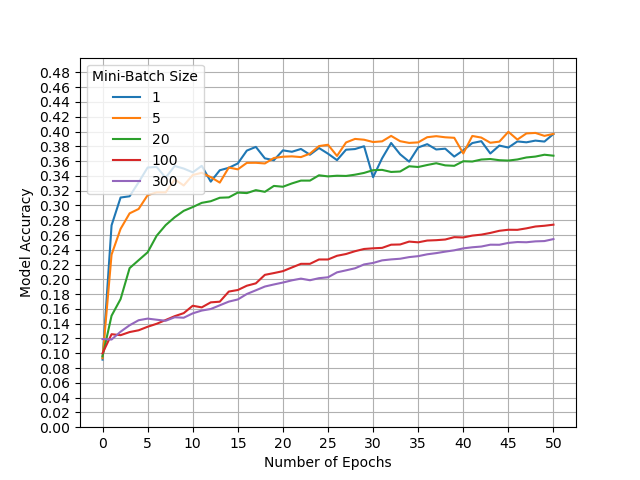
\includegraphics[width=\textwidth]{figures/mbs_cmp.png}
    \caption{
        Effect of mini-batch size on accuracy over epochs \\
        learning rate = 0.1
    }\label{Figure_1}
\end{figure}

\begin{figure}[h!]
    \centering
    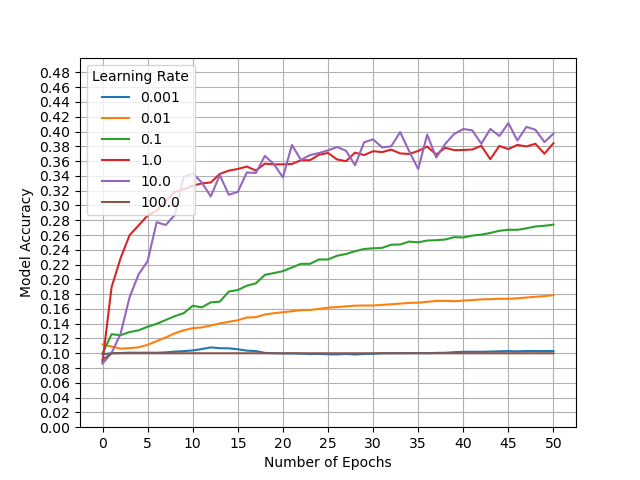
\includegraphics[width=\textwidth]{figures/lr_cmp.png}
    \caption{
        Effect of learning rate on accuracy over epochs \\
        mini-batch size = 100
    }\label{Figure_2}
\end{figure}

\newpage

\subsection{Findings}
\paragraph{Mini-Batch Size}
Mini-batch size has a significant effect on how quickly the error is
reduced. A lower mini-batch size tends to provide faster, but more
erratic error reduction, wheras a higher mini-batch size yields a more
gradual reduction in error due to the gradient vector taking more of the
overall dataset into account. Interestingly, a high mini-batch size
results in any given epoch being much more likely to have a lower error
than the epoch preceding it, although at the cost of training time.

One method to take advantage of this information may be to train the
network for some number of epochs using a much lower mini-batch size.
After which the training can continue using a higher mini-batch size,
allowing the total error to reduce quickly at the beggining and then
more smoothly over time.


\paragraph{Learning Rate}
Learning rate also has a great effect on the rate of error reduction
over epochs. Its effect is similar to that of mini-batch size, with the
major difference being that too high or too low of a learning rate
appears to trap the model in a local optimum. Inside the range of
learning rates which do not trap the model in a local optimum, a lower
learning rate produces a more gradual decrease in error. Likewise, a
higher learning rate tends to decrease the error more rapidly but also
more erratically.

It may also be possible to take advantage of this, too. By training the
network using a high learning rate for some number of epochs and then
switching to a lower learning rate, a more accurate model may be reached
sooner than by using a lower learning rate alone.


\paragraph{Variable Mini-Batch Size and Learning Rate}
By taking advantage of the information learned from the above
experiments, we make estimate when the optimal time to change both
the mini-batch size and learning rate in order to train a model faster.

A mini-batch size of 1 decreases the total error rapidly until
approximately epoch 5 (\autoref{Figure_1}).
Similarly, a learning rate of 10 decreases the error rapidly until
approximately epoch 15 (\autoref{Figure_2}).
By taking advantage of this information and varying the mini-batch size
and learning rate we can train a model with the same accuracy in much
less time. Firstly, we begin training with a mini-batch size of 1 and a
learning rate of 10. At epoch 5 we increase the mini-batch size to 20
and at epoch 10 we decrease the learning rate to 0.1.

This yields the following result

\begin{figure}[h!]
    \centering
    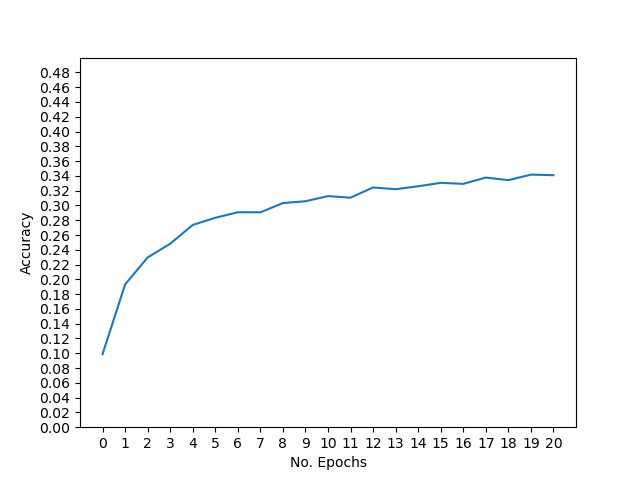
\includegraphics[width=\textwidth]{figures/lr_3.png}
    \caption{ 
        Taking advantage of stuff 
    }\label{Figure_3}
\end{figure}
